\documentclass[letterpaper]{article}
\usepackage{amssymb}
\usepackage{fullpage}
\usepackage{amsmath}
\usepackage{epsfig,float,alltt}
\usepackage{psfrag,xr}
\usepackage[T1]{fontenc}
\usepackage{url}
\usepackage{float}

\begin{document}

\newcommand{\trace}{\mathrm{trace}}
\newcommand{\real}{\mathbb R}  % real numbers  {I\!\!R}
\newcommand{\nat}{\mathbb R}   % Natural numbers {I\!\!N}
\newcommand{\cp}{\mathbb C}    % complex numbers  {I\!\!\!\!C}
\newcommand{\ds}{\displaystyle}
\newcommand{\mf}[2]{\frac{\ds #1}{\ds #2}}
\newcommand{\book}[2]{{Luenberger, Page~#1, }{Prob.~#2}}
\newcommand{\spanof}[1]{\textrm{span} \{ #1 \}}
\parindent 0pt


\begin{center}
{\large \bf HW \# 09 Solutions}
\end{center}

\vspace*{1cm}

\begin{enumerate}
%Prob. 1   Under determined continued
\item \noindent \textbf{Problem 1:} From HW\#8, Prob. 6,
$$ f^{*}=\sum_{i=1}^{n} \beta_{i} y{i}$$
where
$$ \left[\begin{array}{cccc}  <y_1, y_1>&    <y_2, y_1> & \cdots &  <y_p, y_1>\\    <y_1, y_2>&  <y_2, y_2> & \cdots &  <y_p, y_2>
\\
\vdots&   \vdots & \ddots &  \vdots
\\
<y_1, y_p>&    <y_2, y_p> & \cdots &  <y_p, y_p>\end{array} \right]  \left[\begin{array}{c} \beta_1 \\ \beta_2 \\ \vdots \\ \beta_p\end{array} \right] =  \left[\begin{array}{c} c_1 \\c_2 \\ \vdots \\ c_p \end{array} \right] $$
\begin{enumerate}
\setlength{\itemsep}{.1in}
\renewcommand{\labelenumi}{(\alph{enumi})}
\item We have only 1 constraint, and thus $f^{*}=\beta \cdot t$, where
$$<t,t>\beta = 2$$
$$<t,t>=\int_0^{2}\tau^{2}d \tau = \frac{\tau^{3}}{3}\Big|_{0}^2=\frac{8}{3}$$
$$\therefore \frac{8}{3} \cdot \beta = 2 \Rightarrow \beta = \frac{3}{4}$$
$$\therefore \boxed{f^{*} = \frac{3}{4} t}$$

\item We have 2 constraints, and thus
$$ \left[\begin{array}{cccc}  <t, t> & <t, \sin(\pi t)>\\
<t, \sin(\pi t)> & <\sin(\pi t), \sin(\pi t)>\end{array} \right]  \left[\begin{array}{c} \beta_1 \\ \beta_2 \end{array} \right] =  \left[\begin{array}{c} 2 \\ \pi \end{array} \right] $$
$$\begin{aligned}
<t,t>&=\frac{8}{3}~~~~~~\text{from part(a)} \\
<t,\sin(\pi t)> &= \int_0^{2} \tau \sin(\pi \tau) d \tau = -\frac{2}{\pi}\\
<\sin(\pi t),\sin(\pi t)>&=\int_0^{2}\sin^2 (\pi \tau) d \tau = 1
\end{aligned}$$
$$\therefore
\left[\begin{array}{rr} \dfrac{8}{3} &-\dfrac{2}{\pi} \\[2ex]
-\dfrac{2}{\pi} & 1\end{array}\right]
\left[\begin{array}{c}\beta_1 \\ \beta_2\end{array}\right]
=\left[\begin{array}{c}2 \\ \pi\end{array}\right]$$

$$\begin{aligned}
\beta_1&=\frac{3 \pi^2}{2 \pi^2 - 3} \\
\beta_2&=\frac{\pi (2 \pi^2+3)}{2 \pi^2 -3} \\
f^{*}&=\frac{3 \pi^2}{2 \pi^2-3}t+\frac{\pi(2 \pi^2+3)}{2 \pi^2-3}\sin(\pi t)
\end{aligned}$$
\end{enumerate}

\newpage
%Prob. 2   Under determined continued
\item \noindent \textbf{Problem 2:} We define an inner product on $\real^n$ by $<x, \tilde{x}> = x^\top Q \tilde{x}, ~ Q>0$. So that $||x|| = (x^\top Q x)^{1/2}$.\\

\underline{Theorem} If the rows of A are linearly independent, then
$$\hat{x} = \mathrm{arg}~\min_{Ax = b} ||x||$$
is given by
$$\fbox{$\hat{x} = Q^{-1} A^\top (AQ^{-1}A^\top)^{-1} b$} $$

\underline{Proof} We decompose $A$ into its rows, that is  $A=\begin{bmatrix}a_1 \\ \vdots \\ a_m \end{bmatrix}$. Define $\tilde{A} = AQ^{-1}$ and define
$v_i \in \real^n $ by
$v_i = (a_i Q^{-1})^\top = Q^{-1} a_i^\top,$
where we have used the fact that $Q$ is symmetric. It follows that
$$Ax = b \iff <v_i, ~x> = b_i, ~~ i = 1,...,p$$
Hence,
$$\hat{x} = x^* = \sum \limits_{i=1}^{p} \beta_i v_i = [v_1 |~ ... ~|v_p] \beta$$ where $G \beta = b$ and $G$ is the Gram matrix.\\

\underline{Claim} $$G = AQ^{-1}A^\top~~~~~\text{and}~~~~~~[v_1 | ~... ~|v_p] = Q^{-1}A^\top$$  $\hfill \square$

Hence,
$$\hat{x} = Q^{-1}A^\top(AQ^{-1}A^\top)^{-1}b$$ $\hfill \square$

\underline{Proof of Claim:}
$$\begin{aligned} v_i &= Q^{-1} a_i^\top\\
[v_1 | ~... ~|v_p]  &= [Q^{-1}a_1^\top | ... | Q^{-1}a_p^\top]\\
&= Q^{-1}[a_1^\top | ... | a_p^\top]\\
&= Q^{-1} A^\top
\end{aligned}$$


$$\begin{aligned}
G_{ij} &= <v_i, ~v_j>\\
&= v_i^\top Q v_j\\
&= (a_i Q^{-1})QQ^{-1} a_j^\top\\
&= a_i Q^{-1} a_j^\top
\end{aligned}$$

$$\begin{aligned}(AQ^{-1}A^\top)_{ij} &= a_i (Q^{-1} A^\top)_{\text{j-column}}\\
&= a_i Q^{-1} a_j^\top \end{aligned}$$
$\hfill \square$

%Prob. 3 QR
\item \noindent \textbf{Problem 3:}
\noindent \underline{Classical Gram Schmidt} applied to the columns of $A=[A_1, A_2]$ yields orthonormal $\{v^1, v^2 \}$, which when placed as the columns of an orthogonal matrix yield
$$Q=\left[ \begin{array}{rr}0.169& 0.897\\0.507& 0.276\\0.845& -0.345\end{array} \right],$$
The defining $R_{ij} = <v^i,A_j>$ completes the $QR$ factorization developped in lecture:
$$R=\left[ \begin{array}{rr}5.916& 7.434\\0.000& 0.828\end{array} \right].$$
Note that in general (written this way to cover all cases in this problem)
$$A_j = \sum_{i=1}^{\text{number columns of }Q } R_{ij} v^i$$

\noindent \underline{\texttt{[Q,R]=qr(A)}} in MATLAB produces
$$Q=\left[ \begin{array}{rrr}-0.169& 0.897& 0.408\\-0.507& 0.276& -0.817\\-0.845& -0.345& 0.408\end{array} \right]$$
and
$$R=\left[ \begin{array}{rr}-5.916& -7.437\\0.000&0.828\\0.000& 0.000\end{array} \right],$$
while,
\noindent \underline{\texttt{[Q,R]=qr(A,0)}}, the ``economy version'' produces
$$Q=\left[ \begin{array}{rr}-0.169& 0.897\\-0.507& 0.276\\-0.845& -0.345\end{array} \right],$$
and
$$R=\left[ \begin{array}{rr}-5.916& -7.437\\0.000& 0.828\end{array} \right].$$

\textbf{Comparison:}  The economy version of the \texttt{qr} command produces an orthonormal basis for the column span of $A$, just as we did in class. The signs of the orthonormal vectors may be different, but otherwise, the resulting factorization is identical to what we did in lecture.

The ``full'' version of the \texttt{qr} command produces an orthonormal basis for the \textit{co-domain} of $A$. Since $A$ maps $\real^2 \to \real^3$, the command \texttt{[Q,R]=qr(A)} produces an orthonormal basis for $\real^3$;  the first two columns are identical to the vectors produced by the command \texttt{[Q,R]=qr(A,0)} . The matrix $R$ has an extra row of zeros because each column of $A$ is now being expanded in terms of 3 vectors instead of 2. In general, if $A$ maps $\real^n \to \real^m$, then \texttt{[Q,R]=qr(A)} produces an orthonormal basis for $\real^m$, and then $R$ must be such that $QR=A$.


%Prob. 4 QR

%Prob.4
\item \noindent \textbf{Problem 4:} In HW2, Prob 7(b), we set $M=A^{\top}A$, which is symmetric. We deduce that
    $$\min_{x^\top x=1} x^\top A^\top A x = \lambda_{\min}(A^\top A)$$
and
$$\text{arg} \min_{x^\top x = 1} x^\top A^\top A x =v_{\min}$$
where $v_{\min}$ is an e-vector of $A^\top A$ corresponding to the e-value $\lambda_{\min}$, i.e. $A^\top A v_{\min} =\lambda_{\min} v_{\min}$. \\
Moreover, the length of $v_{\min}$ must be chosen to be 1 to satisfy
$$v_{\min}^{\top} v_{\min} = 1$$
From lecture, the columns of $V$ are orthonormal e-vectors of $A^\top A$, arranged so that the e-values of $A^\top A$ are in decreasing order! Hence, $v_{\min}$ is the LAST column of $V$.

%Prob 6
\item \noindent \textbf{Problem 6:} Let $[U,S,V]=\text{SVD}(A)$; that is
$$A=USV^\top$$
with $U$ and $V$ orthogonal, $S$ is diagonal. From page 13 of the SVD handout,
$$\widehat{A} = UDV^\top$$
where
$D=\left[\begin{array}{ccc}\sigma_1 & 0 & 0\\ 0 & \sigma_2 & 0 \\ 0 & 0 & 0\end{array}\right]$
and
$S=\left[\begin{array}{ccc}\sigma_1 & 0 & 0\\ 0 & \sigma_2 & 0 \\ 0 & 0 & \sigma_3\end{array}\right]$ \\[2ex]
Doing the calculations in Matlab yields
$$\widehat{A} =\left[ \begin{array}{rrr}4.042& 7.045& 3.015\\10.043& 17.034& 7.025\\16.008& 27.003& 11.049\end{array} \right].$$

Evaluating the SVD of $\widehat{A}$, per
\begin{verbatim}
[U,S,V]=svd(Ahat);
\end{verbatim}
gives
$$ S=\left[ \begin{array}{rrr}40.285& 0.000&0.000\\0.000&0.186& 0.000\\0.000& 0.000& 0.000\end{array} \right]$$
as expected.

\newpage

%Prob 6: Image compression %Use SVD for something cool.
\item \noindent \textbf{Problem 6:}
\begin{enumerate}
\setlength{\itemsep}{.1in}
\renewcommand{\labelenumi}{(\alph{enumi})}

\item With \texttt{B=double(A)} as in the problem statement, we do \texttt{[U,S,V]=svd(B)}. The plot of the singular values, given by \texttt{diag(s)}, shows that the singular values decrease rapidly.
\begin{center}
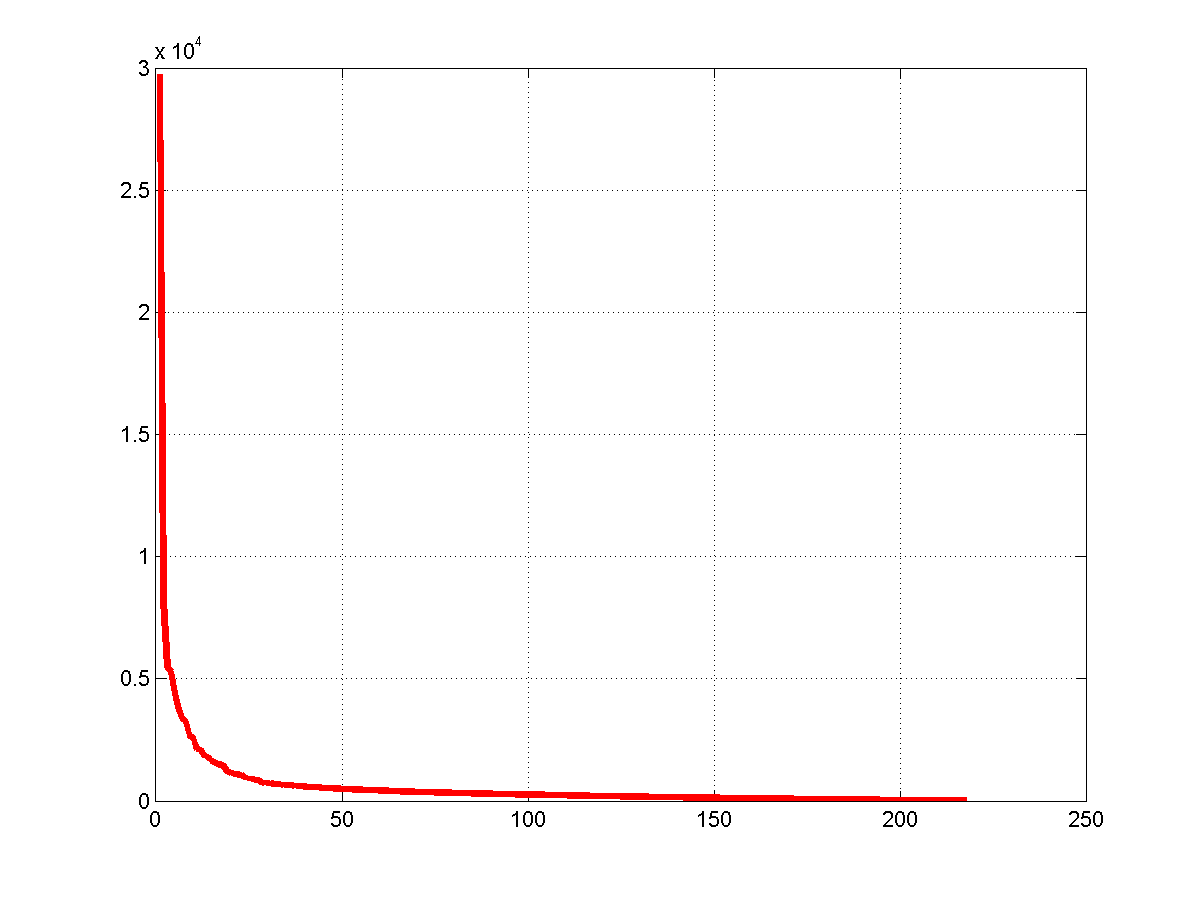
\includegraphics[width=0.6\textwidth]{../MATLAB/SingularValues.png}
\end{center}
Four images were generated accounting for "100\%","90\%","75\%","50\%" of the area under the curve. For example
\begin{verbatim}
    IntegSingVal=cumsum(diag(s));
    K=IntegSingVal(end);
    k2=find(IntegSingVal>.9*K);
    k2=min(k2);
    C2=U(:,1:k2)*S(1:k2,:)*V(1:k2,:)';
\end{verbatim}
Gives k2=99 and the second image. You do not need to do anything fancy! Just playing around is fine.
\begin{center}
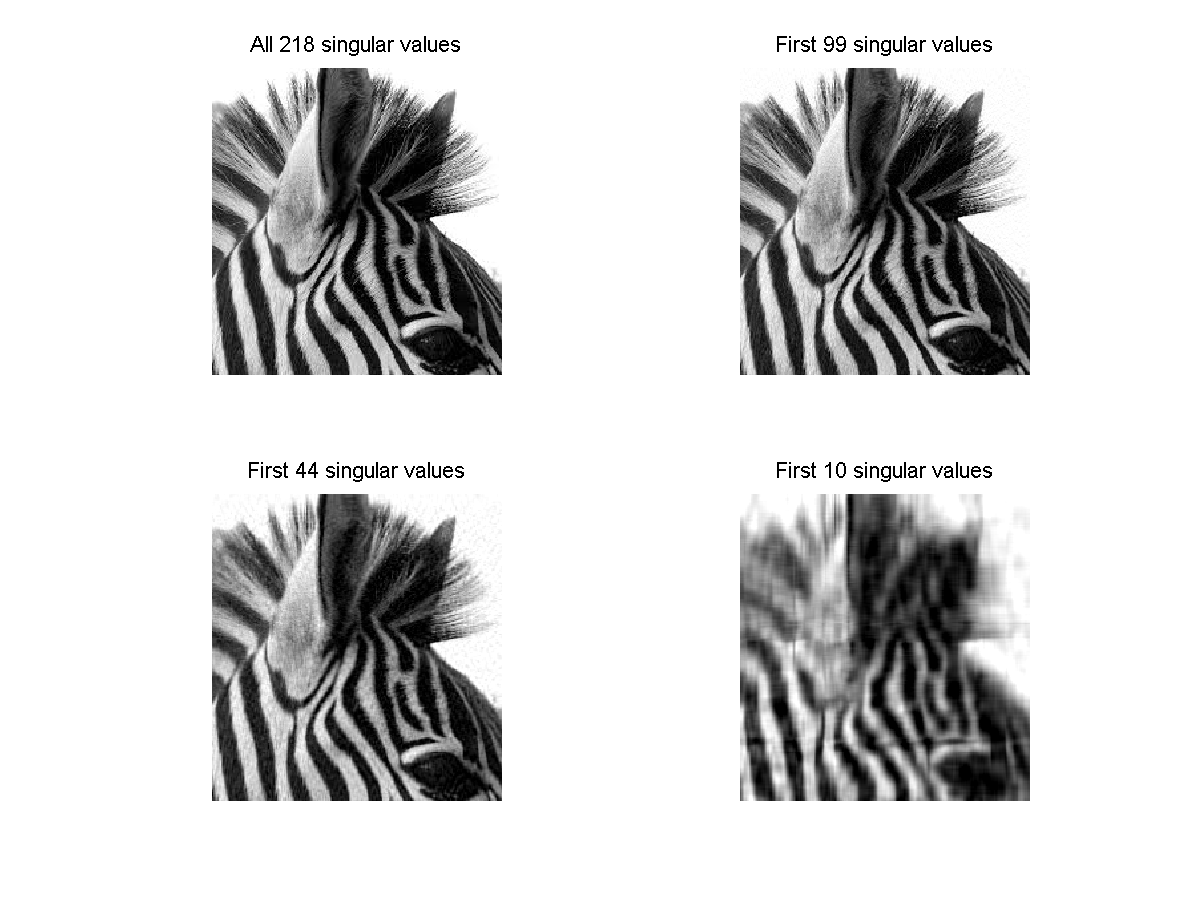
\includegraphics[width=0.7\textwidth]{../MATLAB/FourZebraImages.png}
\end{center}

\item Anything is fine.
\end{enumerate}

%Prob 7
\item \noindent \textbf{Problem 7:}

\begin{enumerate}
\setlength{\itemsep}{.1in}
\renewcommand{\labelenumi}{(\alph{enumi})}
\item The Jacobian is $\frac{\partial f (x)}{\partial x}=\left[   - 3x_3^3 + 6x_2, \frac{4}{3}x_2^3 + 6 x_1, -9x_1x_3^2 \right]$ and
$$\left.  \frac{\partial f (x)}{\partial x}\right|_{x^*} = [ 21, 42, -9]$$
\begin{verbatim}
    syms x1 x2 x3
    x=[x1 x2 x3];
    f=3*x1*(2*x2-x3^3) + (x2^4)/3;
    dfdx=jacobian(f,x);
    dfdx=simple(dfdx)
    latex(dfdx)

    x1=1; x2=3; x3=-1;
    subs(dfdx)
\end{verbatim}

\item  There is no right answer on the choice of $\delta$. I tried $\delta=0.01$ and obtained
\begin{verbatim}
dfdx1 =   2.1000e+01
dfdx2 =   4.2000e+01
dfdx3 =  -9.0003e+00
\end{verbatim}
I also tried $\delta=0.05$ and obtained
\begin{verbatim}
dfdx1 =   2.1000e+01
dfdx2 =   4.2010e+01
dfdx3 =  -9.0075e+00
  \end{verbatim}
  which looks good too!

\item Hiding the function via the encryption tools in MATLAB was pretty cool, no? Iterating on the size of $\delta$ yields
$$ \left.  \frac{\partial f (x)}{\partial x}\right|_{x^*}=  [ 117.3524~~  -41.3685 ~~-636.6017   ~~-3.8520  ~~-11.2049]$$
with $$ \delta = [ 7.6294e-06  ~~ 7.6294e-06   ~~7.6294e-06  ~~ 7.6294e-06   ~~7.6294e-06].$$

Here is my MATLAB code. I used a WHILE loop and a FOR loop to make everything compact. Note how the standard basis vectors were generated as rows of the identity matrix (would have done columns if I had made my $x_0$ a column vector).

\begin{verbatim}
        err_max=1;
        E=eye(5);
        dfdx=zeros(1,5);
        x0=[1 1 1 1 1];
        delta=1*[1 1 1 1 1];
        while err_max>1e-4
            delta=delta/2;
            dfdx_prev=dfdx;
            for k=1:5
                dfdx(k)=( funcPartC(x0+delta(k)*E(k,:)) -  ...
                funcPartC(x0-delta(k)*E(k,:)) )/2/delta(k);
            end
            error = dfdx-dfdx_prev
            err_max=max(abs(error));
        end

        delta
        dfdx
\end{verbatim}


\end{enumerate}


%Prob 8 - Kalman Filter one step
\item \noindent \textbf{Problem 8:}\\
\textit{Prediction Step:}
\begin{align}
\hat x_{1|0}= \hat x_{0|0} + \delta_t \hat u_{1} = 1 + 0.1 \times 10 = 2\nonumber \\ \nonumber\\
P_{1|0} =  P_{0|0}  + \delta_t \times R \times  \delta_t= 0.25 ~+~ 0.1 \times 16 \times 0.1= 0.41 \nonumber 
\end{align}
\textit{Measurement Update Step:}
\begin{align}
K_{1} = P_{1|0} C^\top (C P_{1|0} C^\top + Q)^{-1}= 0.41 \times \frac{-2}{c} \times (\frac{-2}{c} \times 0.41 \times \frac{-2}{c} +10^{-18})^{-1} = -1.422 \times 10^8 \nonumber \\
\hat z_{1|0} = \frac{2}{c}(5-\hat x_{1|0}) = \frac{2}{3 \times 10^8}(5- 2) = 2 \times 10^{-8}\nonumber \\
\hat x_{1|1}= \hat x_{1|0} + K_{1}(z_{1} - \hat z_{1|0}) = 2 -1.422 \times 10^8 \times(2.2 \times 10^{-8} - 2 \times 10^{-8}) = 1.7156\nonumber \\
P_{1|1} = P_{1|0} -  K_{1} C P_{1|0} = 0.41 -  (-1.422) \times 10^8 * \frac{-2}{3 \times 10^8} = \times 0.41 = 0.0213 \nonumber 
\end{align}

Assembling everything together, the state $x_1$ can now be estimated as $ x_1 \sim \mathcal{N}(1.71	56~,~ 0.0213)$.\\

\textbf{Note 1:} In this problem, we trust the sensor measurement a lot and hence you can see that the covariance has decreased a lot. You can try $Q= 10^{-17}$ and see how the state estimate, $x_1$ changes. 
	
\textbf{Note 2:} $P_{1|1}$ is always less than $P_{1|0}$, otherwise, you would not be using the filter! 
\end{enumerate}
\end{document}
